\documentclass[11pt,a4paper]{article}

\usepackage[utf8]{inputenc}
\usepackage[T1]{fontenc}
\usepackage{lmodern}
\usepackage[margin=1in]{geometry}
\usepackage{amsmath,amssymb}
\usepackage{microtype}
\usepackage{enumitem}
\usepackage{booktabs}
\usepackage{tikz}
\usetikzlibrary{arrows.meta,positioning,calc,decorations.pathmorphing,fit,backgrounds}
\usepackage{xcolor}
\usepackage{titlesec}
\usepackage{abstract}
\usepackage{hyperref}
\hypersetup{
  colorlinks=true,
  linkcolor=black,
  urlcolor=blue!50!black,
  citecolor=black
}

% -- palette
\definecolor{ink}{HTML}{0C1220}
\definecolor{amber}{HTML}{C88A2A}
\definecolor{cyan}{HTML}{2A88A0}
\definecolor{brick}{HTML}{B8332E}
\definecolor{slate}{HTML}{4A5468}
\definecolor{paper2}{HTML}{F3F1EC}

\titleformat{\section}{\Large\bfseries\color{ink}}{\thesection}{0.6em}{}
\titleformat{\subsection}{\large\bfseries\color{ink}}{\thesubsection}{0.6em}{}

\renewcommand{\abstractnamefont}{\normalfont\bfseries}
\renewcommand{\abstracttextfont}{\normalfont\small}

\title{\bfseries Classifying Emergence by Information-Flow Operations\\
on the Path Landscape}
\author{[Author Name]\thanks{Correspondence: \texttt{author@institution.edu}.}\\
\small Department / Institution}
\date{\today}

\begin{document}
\maketitle

\begin{abstract}
\noindent
Emergence is ubiquitous across physics, biology, neuroscience, and
artificial intelligence, yet existing classifications remain either
substrate-specific or restricted to coarse weak / strong dichotomies.
We introduce the \emph{path landscape} --- a representation of a
system's information flow as the distribution of input-to-output paths
through its (possibly recurrent, multi-scale) connectivity, grouped
into similarity modes. Within this representation, emergence is not a
property of any single path; it is the visible signature of how the
\emph{distribution} of paths is organized between fixed inputs and
fixed outputs. We argue that every emergent phenomenon can be read as
a combination of four primitive operations on this distribution:
\textbf{path activation}, \textbf{path suppression}, \textbf{mode merge},
and \textbf{mode split}. These four operations form a $2\times 2$
algebra (paths vs.\ groups $\times$ creation/fusion vs.\
removal/fission). Each produces a qualitatively distinct kind of
emergence at the output --- the arrival of new capability, selective
focusing, feature collapse / global integration, and feature
differentiation, respectively. We illustrate the framework with ten
emergent phenomena drawn from ferromagnetism, B\'enard convection,
speciation, cell differentiation, flocking, categorical perception,
working memory, edge detection, grokking in neural networks, and
pidgin-to-creole language formation, showing that the classification
covers diverse fields and accommodates natural mixtures.
\end{abstract}

% =========================================================
\section{Introduction}
% =========================================================

Emergence --- the appearance, at some macroscopic level of a system,
of properties that are not visible at the level of its parts --- is
ubiquitous, but it has resisted a mechanism-grounded classification.
Existing taxonomies either partition emergence by substrate
(``physical'', ``biological'', ``cognitive'') or by epistemic
strength (``weak'' vs.\ ``strong''), neither of which exposes
\emph{how} the underlying machinery actually produces the emergent
output.

In this paper we approach the problem from the side of \emph{information
flow}. Given a system with identifiable inputs and identifiable
outputs, we represent the system by the distribution of routes that
information takes from one to the other. We call this the
\emph{path landscape}. We then ask: what are the qualitatively
distinct ways in which this distribution can be organized so that
the output looks emergent?

The central claim of the paper is that there are exactly four:
information-processing circuits can come online (\textbf{activation}),
existing circuits can be silenced (\textbf{suppression}), groups of
similar routes can fuse (\textbf{merge}), or one group can fission
into several (\textbf{split}). Each operation has a clean structural
fingerprint and a recognizable emergent signature. Together they
form a small algebra in which we believe every emergent phenomenon
can be located, either as a dominant operation or as a mixture.

% =========================================================
\section{The path landscape}
% =========================================================

\subsection{Definition}

Consider any system that can be cast as a directed graph $G=(V,E)$
of \emph{computing units} $V$ connected by \emph{interactions}
$E$. Each interaction carries a (possibly continuous) weight
$w_{uv}\in\mathbb{R}$, and may be feed-forward or recurrent.
Distinguish a set of input units $V_{\text{in}}\subset V$ and a set
of output units $V_{\text{out}}\subset V$. The remaining units are
internal.

If $G$ contains recurrent edges, unroll it in time over $T$
discrete steps, producing the static DAG
$G^{(T)}$ in which each unit $u$ becomes a copy $u\!@\!t$ for
$t=1,\dots,T$, and each recurrent edge $u\!\to\!v$ becomes a
forward-only edge $u\!@\!t \to v\!@\!(t{+}1)$. The unrolled graph
$G^{(T)}$ has no loops by construction.

A \emph{path} from input to output is an ordered sequence of nodes
\[
\pi \;=\; (s_1,\, s_2,\, \dots,\, s_L), \qquad
s_1\in V_{\text{in}},\quad s_L\in V_{\text{out}},
\]
with each $(s_i,s_{i+1})$ an edge of $G^{(T)}$.
We assign to $\pi$ a non-negative weight $\omega(\pi)$ that combines
the magnitudes of the edges it traverses (e.g.\ a product or a normalised
flow). Let $\Pi$ be the set of all such paths.

\subsection{Routes and modes}

Many paths in $\Pi$ differ only in time-step bookkeeping
($u\!@\!t$ vs.\ $u\!@\!t'$) or in a brief lingering on a self-loop.
Stripping these gives a \emph{route} --- the base sequence of
distinct units. Let $R$ be the set of routes. Each route $r\in R$
inherits the cumulative weight of the paths that collapsed onto it.

Two routes are \emph{similar} if they share many of the same units
and edges; for instance, a composite of edge-Jaccard overlap and an
ordered longest-common-subsequence measure. Clustering $R$ under
this similarity produces \emph{modes}: equivalence classes of routes
that compute essentially the same function. The set of modes
$M = \{m_1, m_2, \dots, m_k\}$, together with the route weights, is
the \emph{path landscape}:
\[
\mathcal{L}(G,V_{\text{in}},V_{\text{out}})
\;=\;
\Bigl(\, R,\; \{\omega(r)\}_{r\in R},\; M\,\Bigr).
\]
Three numbers summarize the landscape at a glance: the number of
routes $|R|$, the number of modes $|M|$, and the rank-distribution
of total mode weight.

\subsection{What the landscape sees}

This representation is structural, but it absorbs much of the
continuous dynamics one might fear it discards. Weight magnitudes,
synaptic gains, and effective couplings are encoded in $\omega(r)$.
Coherence, phase relationships, and dynamical co-activation are
encoded in the similarity structure that defines $M$: paths that
fire together over time become close in the similarity metric and
collapse into the same mode. A continuous attractor, for example,
appears as a band of nearly-identical high-weight routes whose
similarity matrix is approximately block-rank-one. Gain modulation
appears as a re-shaping of the weight rank-distribution without a
change of topology.

\subsection{Examples of systems}

\begin{itemize}[leftmargin=*]
  \item \emph{A neural circuit} --- units are neurons or
  micro-circuits, interactions are synaptic connections, recurrence
  is structural feedback, inputs are sensory afferents, outputs are
  motor or downstream targets.
  \item \emph{A deep neural network} --- units are channels or
  attention heads, interactions are weight matrices, inputs are the
  embedding layer, outputs are the prediction head.
  \item \emph{A biochemical regulatory network} --- units are genes
  or metabolites, interactions are regulatory edges, inputs are
  external signals, outputs are phenotypic markers.
  \item \emph{A flock} --- units are birds, interactions are
  near-neighbor coupling, inputs are environmental cues, outputs
  are collective motion.
  \item \emph{A magnetic lattice} --- units are spins, interactions
  are exchange couplings, ``input'' is the boundary condition or
  external field, ``output'' is the macroscopic magnetization.
\end{itemize}

In each case the same definition applies; the differences across
fields are reduced to differences in the structure and weighting
of $\mathcal{L}$.

% =========================================================
\section{Emergence as transformations of the path distribution}
% =========================================================

If a system is fully described by $\mathcal{L}$, then anything that
deserves to be called emergence must be a property of how
$\mathcal{L}$ is organized. We define emergence operationally as a
change in $\mathcal{L}$ that produces a recognizable signature at
the outputs $V_{\text{out}}$.

The transformations of $\mathcal{L}$ have a small irreducible set of
primitives. They are organized along two binary axes (Table~\ref{tab:axes}):
where the change acts (on individual paths, or on groups of paths
--- modes), and the direction of the change (creation/fusion versus
removal/fission).

\begin{table}[h]
\centering
\renewcommand{\arraystretch}{1.25}
\begin{tabular}{lll}
\toprule
 & \textbf{create / fuse} & \textbf{remove / fission}\\
\midrule
\textbf{paths}  & 1. \textbf{Activation} & 2. \textbf{Suppression} \\
\textbf{groups} & 3. \textbf{Mode merge} & 4. \textbf{Mode split} \\
\bottomrule
\end{tabular}
\caption{The four primitive operations on the path landscape.}
\label{tab:axes}
\end{table}

We discuss each in turn, noting both its formal effect on
$\mathcal{L}$ and the emergent signature it produces at the output.
A geographical metaphor, with information flow imagined as a river
shaped by the landscape's geometry, is used throughout to keep the
intuition concrete.

\subsection{Path activation: a new channel opens}

A new route $r\notin R$ becomes viable, either because a previously
silent edge becomes effective or because deeper unrolling reveals a
longer path that traverses a loop. Formally,
$R \to R\cup\{r\}$.

The emergent signature is the \emph{appearance of a new capability}
at the output --- a new behavior, a new representation, a new
qualitative state. The output now does something it could not do
before, because there is now a route along which information of the
required kind can flow.

\textit{Geography.} A new river course is carved: the rain has the
same total volume, but a new path through the terrain becomes
viable, and the lake at the bottom of the basin now receives water
it did not previously receive.

\textit{Recurrent loops as a sub-case.} Recurrence does not require
a new ``time-emergence'' category. In the unrolled graph, a path
that revisits a unit via a feedback edge is simply a longer path,
and it becomes available at a sufficient unrolling depth. The
emergent signature --- persistence, attractor convergence,
iterative refinement --- is then exactly the signature of
activation, applied to a long re-entrant route.

\subsection{Path suppression: a channel is dammed}

An existing route $r\in R$ is silenced: either because of inhibition
along one of its edges, or because of gating that prevents weight
from flowing along it. Formally, $R \to R\setminus\{r\}$, or
equivalently $\omega(r)\to 0$.

The emergent signature is \emph{selective focusing}: the output
becomes sharper not because anything has been added but because
competing flow has been removed. Lateral inhibition produces
edge-like features by suppressing paths that carry the homogeneous
background. Attention picks out a target by suppressing distractor
routes. Signal emerges from noise because noise paths have been
silenced.

\textit{Geography.} A dam is built across a channel: the water that
used to dissipate sideways is now confined to the remaining route,
which becomes recognizable as a sharp downstream feature.

\subsection{Mode merge: a gorge concentrates flow}

Two (or more) modes $m_i, m_j \in M$ fuse into a single mode
$m_{ij}$. Formally, $M \to (M\setminus\{m_i,m_j\})\cup\{m_{ij}\}$
with $\omega(m_{ij}) = \omega(m_i)+\omega(m_j)$.

The emergent signature is \emph{feature collapse and global
integration}: paths that previously computed distinguishable
sub-features now collapse onto a shared output sub-pattern.
Categorical perception, binding, abstraction, holistic
representation, generalization, and the formation of macroscopic
order from microscopic configurations all live here.

\textit{Geography.} The terrain narrows into a gorge: many tributaries
that were running roughly parallel are forced into a single river,
and the downstream observer no longer sees the tributaries
individually --- only the concentrated current.

\subsection{Mode split: a delta spreads flow}

A single mode $m\in M$ fissions into two or more sub-modes
$m_a, m_b, \dots$. Formally, $M \to (M\setminus\{m\})\cup\{m_a,m_b,\dots\}$
with $\omega(m_a)+\omega(m_b)+\cdots = \omega(m)$.

The emergent signature is \emph{feature differentiation}: a
previously uniform output space acquires distinguishable
sub-patterns. Specialization, discrimination, symmetry-breaking,
expert tuning, and the appearance of novel sub-categories all live
here.

\textit{Geography.} The river enters a delta: a single channel
fans out into distinguishable sub-channels, and downstream the
flow is recognized as a structured set of distinct streams rather
than one uniform current.

\subsection{Composition and mixtures}

Real emergent phenomena are rarely pure. Categorical perception
is mostly mode merge (within-category collapse) but contains a
thin admixture of mode split (between-category sharpening).
Grokking is mostly path activation but is followed by a merge in
which the new circuit unifies many examples. Speciation is split
in its dominant operation but is enabled by suppression of
inter-population gene flow. The classification is not a
partition; it is a basis. Every emergent phenomenon decomposes
into a (possibly time-extended) combination of the four
operations.

% =========================================================
\section{Schematic of the four operations}
% =========================================================

Figure~\ref{fig:schematic} sketches the four operations in
side-by-side, low-information form: each panel shows a small input
fan, a few routes through internal units, and a small output fan,
and a thumbnail of the river geography that motivates the name.

\begin{figure}[h]
\centering
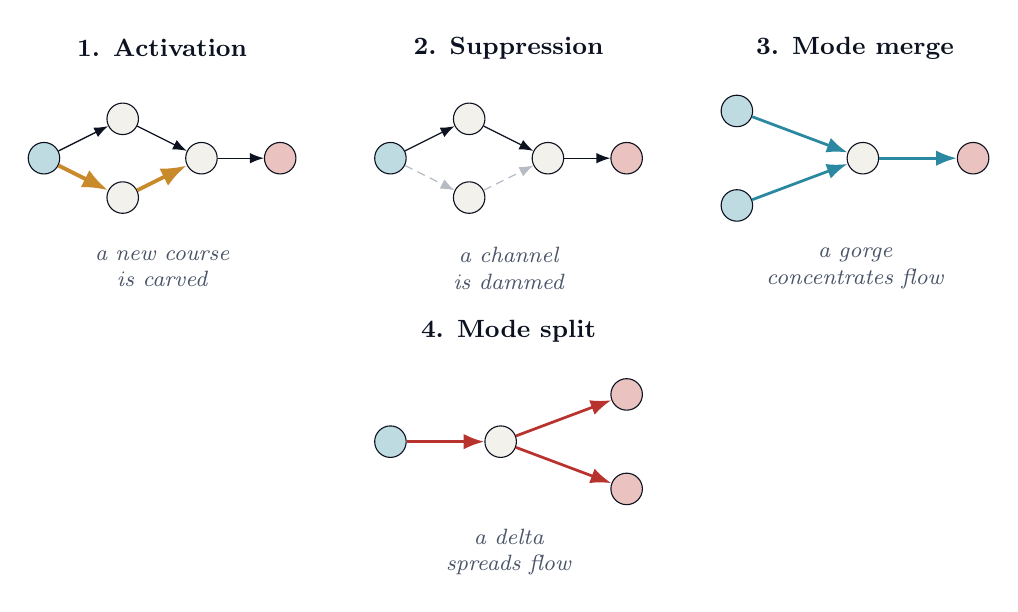
\begin{tikzpicture}[
  every node/.style={font=\small},
  unit/.style={circle, draw=ink, fill=paper2, minimum size=4mm, inner sep=0pt},
  innode/.style ={unit, fill=cyan!30},
  outnode/.style={unit, fill=brick!30},
  arrow/.style={-Latex, line width=0.45pt, color=ink},
  arrow new/.style={-Latex, line width=1.4pt, color=amber},
  arrow off/.style={-Latex, line width=0.45pt, color=slate!40, densely dashed},
  arrow merge/.style={-Latex, line width=1.0pt, color=cyan},
  arrow split/.style={-Latex, line width=1.0pt, color=brick},
  lbl/.style={font=\bfseries\small\color{ink}},
  cap2/.style={font=\footnotesize\itshape\color{slate}, align=center}
]

% --- panel 1: ACTIVATION
\begin{scope}[xshift=0cm]
  \node[innode]  (i)  at (0,1)   {};
  \node[unit](a)  at (1,1.5) {};
  \node[unit](b)  at (1,0.5) {};
  \node[unit](c)  at (2,1)   {};  % the new unit
  \node[outnode] (o)  at (3,1)   {};
  \draw[arrow] (i) -- (a);
  \draw[arrow] (a) -- (c);
  \draw[arrow] (c) -- (o);
  \draw[arrow new] (i) -- (b);     % new path
  \draw[arrow new] (b) -- (c);
  \node[lbl] at (1.5,2.4) {1. Activation};
  \node[cap2]   at (1.5,-0.4) {a new course\\is carved};
\end{scope}

% --- panel 2: SUPPRESSION
\begin{scope}[xshift=4.4cm]
  \node[innode]  (i)  at (0,1)   {};
  \node[unit](a)  at (1,1.5) {};
  \node[unit](b)  at (1,0.5) {};
  \node[unit](c)  at (2,1)   {};
  \node[outnode] (o)  at (3,1)   {};
  \draw[arrow] (i) -- (a);
  \draw[arrow] (a) -- (c);
  \draw[arrow] (c) -- (o);
  \draw[arrow off] (i) -- (b);
  \draw[arrow off] (b) -- (c);
  \node[lbl] at (1.5,2.4) {2. Suppression};
  \node[cap2]   at (1.5,-0.4) {a channel\\is dammed};
\end{scope}

% --- panel 3: MERGE
\begin{scope}[xshift=8.8cm]
  \node[innode]  (i1) at (0,1.6) {};
  \node[innode]  (i2) at (0,0.4) {};
  \node[unit](h)  at (1.6,1) {};
  \node[outnode] (o)  at (3,1)   {};
  \draw[arrow merge] (i1) -- (h);
  \draw[arrow merge] (i2) -- (h);
  \draw[arrow merge] (h)  -- (o);
  \node[lbl] at (1.5,2.4) {3. Mode merge};
  \node[cap2]   at (1.5,-0.4) {a gorge\\concentrates flow};
\end{scope}

% second row
% --- panel 4: SPLIT
\begin{scope}[xshift=4.4cm, yshift=-3.6cm]
  \node[innode]  (i)  at (0,1)   {};
  \node[unit](h)  at (1.4,1) {};
  \node[outnode] (o1) at (3,1.6) {};
  \node[outnode] (o2) at (3,0.4) {};
  \draw[arrow split] (i) -- (h);
  \draw[arrow split] (h) -- (o1);
  \draw[arrow split] (h) -- (o2);
  \node[lbl] at (1.5,2.4) {4. Mode split};
  \node[cap2]   at (1.5,-0.4) {a delta\\spreads flow};
\end{scope}

\end{tikzpicture}
\caption{Schematic of the four primitive operations on the path
landscape. Cyan circles are input units; red circles are output
units. \textbf{Activation} introduces a new route (amber).
\textbf{Suppression} silences an existing route (dashed grey).
\textbf{Mode merge} concentrates routes into a shared sub-pattern.
\textbf{Mode split} fissions one sub-pattern into several. Each
panel is captioned with its river-geography metaphor.}
\label{fig:schematic}
\end{figure}

% =========================================================
\section{Causes: the geography of information flow}
% =========================================================

A useful way to think about \emph{why} a system exhibits one
operation rather than another is to remember that, in the river
metaphor, the operations are not chosen by the water --- they are
imposed by the geography. The path landscape \emph{is} the
geography of the system, and the four operations correspond to
four canonical shapes that the landscape can take.

\paragraph{Why activation occurs.} The system has acquired a new
viable course. In neuroscience this might be the maturation of an
axon tract, in machine learning a circuit that emerged from
gradient descent, in linguistics a regularization performed by
child learners. In each case the cause is a structural change in
the graph $G$, or a deepening of the unrolling $T$, that makes a
new route from input to output possible. \emph{Cause: new
connectivity, or deeper recurrence.}

\paragraph{Why suppression occurs.} The system has installed a
gating mechanism that selectively damps existing routes. In
visual cortex this is lateral inhibition; in attention it is
top-down gain control; in evolutionary biology it is reproductive
isolation. \emph{Cause: inhibitory or gating connectivity that
operates on routes already present in $\mathcal{L}$.}

\paragraph{Why mode merge occurs.} Multiple routes converge in
their structure or in their effective output --- either because
they share intermediate units, because their endpoints coincide,
or because their dynamical activity becomes correlated. In
physics, falling below a critical temperature aligns spins; in
perception, a learning history of equivalent reinforcement
collapses categories. \emph{Cause: shared structure or shared
weighting that forces formerly distinct modes into one.}

\paragraph{Why mode split occurs.} A previously uniform mode is
broken apart by a structural or weighting difference that the
landscape is now sensitive to --- a symmetry-breaking bifurcation,
a developmental signal, a learning experience that introduces a
relevant contrast. \emph{Cause: a structural or weighting
asymmetry that fissions a previously homogeneous mode.}

In all four cases the cause is the same in form: the geometry of
$G$ (together with the unrolling and the weighting) makes a
particular operation on $\mathcal{L}$ inevitable. The cause of
emergence is the cause of the operation that produces it.

% =========================================================
\section{Case studies across fields}
% =========================================================

To illustrate the classification we discuss ten emergent phenomena
drawn from physics, biology, neuroscience, cognitive science,
machine learning, and linguistics. They are grouped by the
dominant operation of the corresponding path-landscape
transformation.

\subsection{Path activation (new capability appears)}

\paragraph{Grokking in neural networks (machine learning).}
After many training steps with apparent overfitting, the model
abruptly generalizes; mechanistic interpretability has identified
that a new internal circuit (for example a Fourier-decomposition
circuit for modular arithmetic) suddenly carries the computation.
A previously dormant route through the weights takes over: this is
path activation in the cleanest sense.

\paragraph{Pidgin-to-creole language formation (linguistics).}
Children exposed to a structurally impoverished pidgin
spontaneously produce a grammatically rich creole, with recursion,
tense, and case-marking that were not present in the input. New
combinatorial routes from intended meaning to spoken sentence
come online that the parent system did not contain.

\paragraph{Working memory persistent activity (neuroscience).}
A stimulus that has physically vanished is held active in
prefrontal circuits for seconds. In the path landscape this is the
recurrent sub-case of activation: longer paths that loop back
through the same units become viable with deeper unrolling, and
emergence appears as sustained re-processing of an absent input.

\subsection{Mode merge (global integration)}

\paragraph{Ferromagnetism below the Curie point (physics).}
Above $T_c$, individual spin-orientation paths are independent;
below $T_c$, the route distribution collapses onto one dominant
aligned mode, and macroscopic magnetization appears as the
integration of microscopic routes.

\paragraph{Categorical perception (cognitive neuroscience).}
A physical continuum (color hue, the /ba/--/pa/ acoustic
continuum) is heard or seen as discrete categories with sharp
boundaries. Many input routes (small stimulus variations) merge
onto the same output mode: the percept is the merge.

\paragraph{Starling murmurations (collective animal behavior).}
The flight-decision routes of thousands of individual birds become
correlated across the flock. The route distribution acquires a
single coherent collective mode (the flock's direction) that no
single bird's wiring contains.

\subsection{Mode split (feature differentiation)}

\paragraph{Speciation (evolutionary biology).}
One ancestral gene-flow cluster fissions into two reproductively
isolated populations, each carving out its own route through
morphological and behavioral space.

\paragraph{Cell differentiation (developmental biology).}
A pluripotent stem cell, whose gene-regulatory routes form a
single cluster, fissions into many specialized cell-type
clusters --- neurons, hepatocytes, myocytes --- each tracing a
distinct regulatory route through the same genome.

\paragraph{B\'enard convection cells (nonlinear physics).}
A uniform fluid heated from below has homogeneous flow paths;
above a critical temperature gradient the route distribution
fissions into ordered convection cells with distinct upflow and
downflow lanes. Symmetry-breaking is, structurally, mode split.

\subsection{Path suppression (selective focusing)}

\paragraph{Edge detection in V1 by lateral inhibition (vision).}
Center--surround receptive fields actively suppress paths from
neighboring photoreceptors at regions of uniform luminance,
leaving only paths at luminance discontinuities active. Edges
appear not because edge-routes were added but because
background-routes were silenced.

A quick reading of the distribution: physics and developmental
phenomena tend to live in split (symmetry-breaking,
differentiation); collective and perceptual phenomena tend to
live in merge (binding, alignment, categorization);
novelty-and-skill phenomena live in activation (new circuits,
persistent activity); attention-and-feature-detection phenomena
live in suppression. Most real cases are dominated by one
operation but contain a thin admixture of the others, which is
exactly what a four-operation algebra should predict.

% =========================================================
\section{Discussion}
% =========================================================

\subsection{What the framework gains}

Three things follow from treating emergence as transformation of
the path distribution. First, the classification is
mechanism-grounded: an instance of emergence is named by the
operation that produced it, not by the substrate in which it lives.
Second, the framework is field-agnostic --- once a system can be
written as a directed graph with inputs and outputs, its
emergent behavior is comparable to that of any other such system.
Third, recurrence and time fold into the framework without a
separate axis: a recurrent loop is just a longer path that
becomes active at a sufficient unrolling depth, so persistence
and oscillation are sub-cases of activation rather than a
parallel taxonomy.

\subsection{Limits of the structural view}

The path landscape is a projection. It absorbs continuous
dynamics through path weights and inter-route similarity, but
phenomena whose essence lives in the magnitude of a single signal
or in the phase of a continuous oscillation are visible only as a
coarse shadow. The framework is therefore most informative for
emergent phenomena whose primary content is the
\emph{organization} of information flow, and least informative
for those whose primary content is the raw amplitude or
high-resolution phase of the flow.

\subsection{Predictions and falsifiability}

Because the operations are defined structurally, they make
testable predictions. For example: if a system's emergence is
classified as merge, a targeted lesion of any of the
intermediate units shared across the merging routes should
abolish the emergent property; if it is classified as
suppression, restoring the silenced routes (by lifting the
inhibition) should make the emergent feature disappear; if it is
classified as activation, the operation can be turned on and off
by varying the unrolling depth or the connectivity that creates
the new route. The framework is therefore not a relabeling
exercise: it commits to specific causal predictions about which
structural interventions will and will not destroy a given
instance of emergence.

% =========================================================
\section{Conclusion}
% =========================================================

We have argued that emergence, despite its apparent diversity
across fields, factors into a small set of operations on a single
representation: the path landscape. The four primitive operations
--- activation, suppression, merge, and split --- exhaust the
qualitatively distinct ways that the distribution of input-to-output
routes can be transformed, and each produces a recognizable kind
of emergent signature at the output. Real phenomena are typically
dominated by one operation and accompanied by minor admixtures of
the others. The classification is field-agnostic, structurally
grounded, and yields concrete predictions about which interventions
will preserve and which will destroy any given instance of
emergence. We hope it provides a useful common language across
the many disciplines in which emergence is named but rarely
mechanistically classified.

\paragraph{Acknowledgments.} We thank colleagues who pressed on
early versions of the operation algebra, in particular for
insisting that the recurrent / time-extended class be folded into
activation rather than treated separately.

\end{document}
